\documentclass{sigchi-alternate}

% Use this command to override the default ACM copyright statement (e.g. for preprints). 
% Consult the conference website for the camera-ready copyright statement.
%\toappear{%
%Permission to make digital or hard copies of all or part of this work for personal or classroom use is granted without fee provided that copies are not made or distributed for profit or commercial advantage and that copies bear this notice and the full citation on the first page. Copyrights for components of this work owned by others than the author(s) must be honored. Abstracting with credit is permitted. To copy otherwise, or republish, to post on servers or to redistribute to lists, requires prior specific permission and/or a fee. Request permissions from \href{mailto:permission@acm.org}{Permissions@acm.org}.\\[3pt]
%\textit{CHI 2014}, April 26--May 1, Toronto, ON, Canada.\\
%Copyright is held by the owner/author(s). Publication rights licensed to ACM.
%}
%\submissionversion{CHI 14}

% Load basic packages
\usepackage{balance}  % to better equalize the last page
\usepackage{graphicx} % for EPS, load graphicx instead
\usepackage{url}      % llt: nicely formatted URLs
\usepackage[utf8]{inputenc}
\usepackage[toc,page]{appendix}
\usepackage{float}
\usepackage{rotating}

% llt: Define a global style for URLs, rather that the default one
\makeatletter
\def\url@leostyle{%
	\@ifundefined{selectfont}{\def\UrlFont{\sf}}{\def\UrlFont{\small\bf\ttfamily}}}
\makeatother
\urlstyle{leo}

% remove those two lines if you don't want to use biblatex
\usepackage[style=sigchi,backend=biber,doititles]{biblatex}
\addbibresource{references.bib}
%\DeclareBibliographyCategory{ignore}
%\addtocategory{ignore}{AGORAVA}
%\addtocategory{ignore}{CLOUDRAIL}
%\addtocategory{ignore}{SOCIALMEDIA-ABSTRACTIONS}
%\addtocategory{ignore}{ASNE}

% hyperref was already loaded by the documentclass.
% Use nohyperref option to prevent this from happening.
\hypersetup{
	pdftitle={Ingen titel än},
	pdfauthor={LaTeX},
	pdfkeywords={SIGCHI, proceedings, archival format},
	bookmarksnumbered,
	pdfstartview={FitH},
	colorlinks,
	citecolor=black,
	filecolor=black,
	linkcolor=black,
	urlcolor=black,
	breaklinks=true,
}

% create a shortcut to typeset table headings
\newcommand\tabhead[1]{\small\textbf{#1}}

% End of preamble. Here it comes the document.
\begin{document}

% Arabic page numbers for submission. 
% Add this line to eliminate page numbers for the camera ready copy
%\pagestyle{empty}

\title{The feasibility and practicality of a generic social media library}

\numberofauthors{2}
\author{
	\alignauthor{Fredrik Jonsén\\
		\affaddr{Linköping University}\\
		\affaddr{Linköping, Sweden}\\
		\email{frejo105@student.liu.se}}
	\alignauthor{Alexander Stolpe\\
		\affaddr{Linköping University}\\
		\affaddr{Norrköping, Sweden}\\
		\email{alest170@student.liu.se}}
}

\maketitle

\begin{abstract}
Many people today use social media in one way or another, and many of these platforms have released APIs developers can use to integrate social media
in their applications. As many of these platforms share a lot of functionality we see a need for developing a library, to contain these, and ease the
development process when working with the platforms. The purpose of this paper is to find common functionality and explore the possibility of generalization
in this regard. We first look for common denominators between the top social media networks, and using this information we attempt to make an implementation
to evaluate the practicality. After the development process we analyze our findings and discuss the usability and maintainability of such a library.
\end{abstract}

\section{Introduction}
Today a lot of people are using social media in one way or another and it is estimated that there will be around 2.67 billion social media
users around the globe by 2018\autocite{STATISTA_SN_WORLD_USERS}. Most of these social networks have released Application Programming Interfaces (APIs)
which developers can utilize to integrate these networks into their software.

Social network usage is growing and has gone from 0.97 billion users in 2010 to 2.14 billion in 2015\autocite{STATISTA_SN_WORLD_USERS}. This would
account for approximately 29\% of the earth's population in 2015, which was 7.347 billion 2015\autocite{WORLD_BANK_POPULATION}. It is worth noting
that this counts created user accounts and not unique users, one person can have several accounts over multiple networks, and accounts may not
belong to an actual person, but rather companies, organizations, or bots.

Because of the currently high, and still growing, number of social media users we find it highly likely that we will see an increasing number of
applications that involve social media in their software in one way or the other. Out of all the social networks existing today there are twenty
that have more than 100 million active accounts\autocite{STATISTA_LEADING_SOCIAL_NETWORKS}. This means that if we would want to create an application
that involves a lot of social networks we will have to do a lot of work just to implement all of these into our system.

\subsection{Purpose}
Because of this we see a need for a way to combine these social network APIs in some way to save development
time and reduce the amount of duplicate code written in software. The purpose of this project is to create a library 
that combines the APIs in a modular fashion, where each API serves as a module in order to simplify adding new networks,
and make it easier to involve social media in software. 

A software library by definition is a set of pre-written code that a developer might add to a project in order to add more functionality or to ease the 
development process\autocite{TLDP_LIBRARY_DEFINITION}. 

For our study, we define modularity as the extent to which a program can be divided into modules where\autocite{Kiczales:2005:APM:1062455.1062482}
where each module has it's own well-defined interface, and there should be no need to modify the interface when changing the module's actual implementation.
Together, these modules should be easily combined to make up a full program. In the present case modularity will mostly affect how easy it will be to integrate
new social media APIs in the future.
%\begin{itemize}
%	\item Each module has a well-defined interface that describes how the system can interact with it.
%	\item Changes to the underlying functionality of a module does not affect the modules interface.
%	\item Modules can be put together with other modules in different ways to make a complete program
%\end{itemize}%


Over time, as new social networks enter the market, it will have to be possible to integrate them into our library. As such, the code will have to be maintainable.
Maintainability is a very broad term, but in general focuses on how simple the code in itself is to work with, when changes or new additions are necessary.
In the Theory chapter we will explore this subject more thoroughly. For the evaluation of the maintainability of our library, we will be making use of the third
party tool SonarQube\footnote{https://www.sonarqube.org/}.


\section{Research Question}
Is it possible to create a maintainable modular library for social network APIs?

As the question pertains to the \textit{possibility} of creating the library, it is also necessary to define what would make us deem it impossible to finalize
the library with a satisfactory result. In regards to this, we see two major potential risk factors:
\begin{enumerate}
	\item It may not be possible to generalize the results of the APIs, but each API will instead require a large mount of exceptions, making a common interface meaningless.
	\item The rate of changes to the APIs may be unmaintainable. If we during the course of the relatively short development time find ourselves having to go back multiple
	times to adjust already implemented functionality due to changes in the API, we will consider the library unmaintainable.
\end{enumerate}
\section{Limitations}
Because there are so many social networks existing today and we have a finite amount of time to complete this
project we will focus on a smaller set of APIs to implement into our library.  We have set up a few criteria 
for the APIs so we can find suitable candidates for our library, which are:
\begin{itemize}
	\item The social network must be one of the 22 most popular\autocite{STATISTA_LEADING_SOCIAL_NETWORKS}.
	\item It must be relevant for our geographical location, in this case Europe.
\end{itemize}
Other than this we will judge the API itself subjectively by how good its documentation is, its functionality and its ease-of-use. 

\section{Theory}
\subsection{Code Reuse}
A lot of time and money can be saved by reusing code, of which libraries are one form. Although there are
some issues with using libraries, the gains from avoiding reinventing the wheel makes writing and using
libraries a common practice, in particular in open source software\autocite{2998479020080101}.

Writing code which can be easily reused requires a deeper analysis of the problem domain, which may increase the cost and time required compared 
to developing the same code without reuse in mind, but can drastically decrease the cost of developing systems in the future where the code can 
be reused \autocite{lim1994effects}. This cost reduction is apparent foremost in terms of direct cost of development, but also in time-to-market, 
which can be argued to be even more important in the long term\autocite{griss1993software}.

With code reuse there are also several potential issues which have to be kept in mind, both when it comes to the implementation itself but also 
when it comes to using the implementation. Backwards compatibility between versions is a major topic in itself\autocite{raemaekers2012measuring}. There 
is also the risk of a library being abandoned by it’s maintainer. This is especially true for proprietary libraries, where the source code may not 
be available. It this case, the library might have to be replaced, making all the effort to use the library wasted.

\subsection{Library Interface Design}
When designing our library we will want keep several things in mind. We want to design the library so it’s easy and straightforward to use for a 
developer. As Henning points out in his article\autocite{Henning:2007:ADM:1255421.1255422}, about design of APIs, it is very easy to create a bad one, 
but very hard to create an API that feels natural and easy to work with. APIs, as we know, are a kind of interface for a program to gain access to 
another program without direct access, and can be compared to the interface of our library.

Henning continues to discuss guidelines for how an API should generally be designed. What feels most relevant to our work is how 
he describes how the APIs should be designed from the perspective of a user, because when it’s done from the implementer's point of view the 
needs of the user are often forgotten. It’s usually best to document first, because when it is done after the implementation the programmer, who 
wrote the functionality, will usually just dictate what he did, rather than make it is obvious enough for others who are not as familiar with the code.

\subsection{Maintainability}
Maintainability can be defined as the simplicity with which defects can be corrected and the library can be extended or modified to support future 
requirements.\autocite{5733835}. This can generally be measured by certain quantifiable attributes, such as unit test coverage, lines of code and cyclomatic complexity.
\autocite{SONARQUBE_MAINTAINABILITY_DEFINITION}. It also includes more subjective aspects, such as how self-explanatory the code is, and how well commented sections
of necessarily complex code is.

\subsection{Social Media APIs}
A social media API is an interface through which the software can integrate functionality offered by the social media platform, commonly set up as a REST API. 
These can be used through registering the application on the social media site, thus acquiring an authentication token which can be used to call different
endpoints via HTTP. The services offered varies between the APIs, but tend to share some basic functionality such as publishing posts and sending private messages.

As mentioned, one of the biggest issues with using libraries is the risk of the project being abandoned. This risk increases significantly when the library
itself uses APIs which integrate oft-changing platforms, such as the case of Social Media. The rate of change differs between networks, in some cases on average
three times a year\footnote{https://developers.facebook.com/docs/apps/changelog}, in other cases several times a month\footnote{https://www.hitchhq.com/twitter/activities},
although the impact of the changes varies greatly. At best, a lack of active development simply means missing out on new functionality. In other cases, such as 
unfixed security vulnerabilities\footnote{https://github.com/gorbin/ASNE/issues/107}, may render the library unusable.

\subsection{Similiar work}
Several similar works, Agorava\footnote{http://www.agorava.org/}, ASNE\footnote{https://github.com/gorbin/ASNE} and 
SocialMedia Abstractions\footnote{https://github.com/socialsensor/socialmedia-abstractions} serve the same or similar purposes, but all were abandoned before reaching a 
stable release. In the case of ASNE, the project was abandoned explicitly due to a lack of free time. This shows the issue of a library having only a single maintainer, 
as the project risks being abandoned by it's developer as soon the project is no longer a priority. The others have no stated reason for the lack of continued development.
There are also commercial services\footnote{https://cloudrail.com} which provide this functionality for some popular APIs, but charge money to sign up 
and use. As it is proprietary it's inner workings are completely opaque, and thus will not be examined by this study.

\subsubsection{Encountered issues}
Despite being abandoned, we hope the research community can still learn from the problems the similar libraries encountered and solved. For this, we looked into each project's issue
tracking (where available) and commits. This was somewhat complicated in that one project, SocialMedia Abstractions, simply had not used issue tracking. 
Another project, ASNE did use issue tracking, but much of the discussion regarding individual issues was largely in Russian, making it unusable in our case. 
The issues, despite the name, did not always regard bugs. In the vast majority of cases, issued stemmed from users misunderstanding the library documentation,
requesting features, or suggesting refactoring of code to increase maintainability. In the case of documentation misunderstandings, these were often
solved by simply adding examples. There was also a noticeable difference in the amount of issues pertaining bugs in ASNE, which included no automatic tests,
compared to Agorava, which includes a large amount of automatic tests, and had almost no issues regarding logical errors, despite having a much larger code base.

\section{Method}
To find out if we could create a modular library for social network APIs we structured our project into three different parts. We began with evaluating the most 
popular networks on a basis of which are relevant for our project and which are appropriate to integrate into our library based on functionality. As the next step we then implemented
the library, using SonarQube throughout development to ensure code quality and maintainability stayed high. Lastly we evaluated the library in two different ways.
First we analyzed the data we got from SonarQube and see how well our library performs, and then created a small application, in order to test the library's practical usability.

\subsection{Social Networks selection}
To choose which APIs to implement into our library we initially looked at what social media network sites where most popular\autocite{STATISTA_LEADING_SOCIAL_NETWORKS}.
Out of these networks we sorted out those which were geographically irrelevant for the focus of this project, which is the European market. We then further narrowed down
the list by looking at the functionality of each API. We selected the APIs which shared a lot of common functionality, which made them more appropriate for the core idea
of our study, to develop a modular library.

\subsection{Implementation}
When we had chosen APIs to implement we started we started to implement our library. For this we have chosen to work in the Java language, as we found a decent
number of pre-existing API-specific libraries we could use in this language. We used the most current version of Java at the time of our project, Java SE 8. We also used several
tools, which we will describe briefly.
\subsubsection{Maven}
Maven\footnote{https://maven.apache.org/} is a project management tool. While the tool includes a lot of functionality, we mostly made use of its automated build tool, release-, and
dependency management.
\subsubsection{IntelliJ IDEA}
IntelliJ IDEA\footnote{https://www.jetbrains.com/idea/} is the Integrated Development Environment we chose for our project. It offers integration with Maven, syntax highlighting,
static analysis, boilerplate code generation and other functionality to simplify the implementation work.
\subsubsection{Travis CI}
Travis\footnote{https://travis-ci.org/} is a free Open Source service for continuous integration. It integrates with github and runs tests automatically for the project when changes are
checked in. When done, participants of the project can be notified of the result.
\subsubsection{SonarQube}
Sonarqube\footnote{https://www.sonarqube.org/} is a service for, in their own words, continuous code quality. As with Travis, it integrates with GitHub and automatically runs a series of
checks when code is committed to the repository. This includes analysing the code for general issues, such as a high cyclomatic complexity, missing documentation and dead code, but also
more detailed issues which may be easy to miss, such as potential infinite loops, unhandled exceptions, or checking floating point numbers for equality.

\subsection{Work Method}
We chose to work using a test driven development process, where we first wrote tests for our interfaces. During this process we also documented the functionality according to 
Hennings\autocite{Henning:2007:ADM:1255421.1255422} concept of documenting first, in an effort of making the documentation more understandable from the users perspective. During this
period we implemented functionality iteratively for our two prioritized APIs, implementing one functionality at a time for each as to not be left with only one fully implemented API in our library.

\subsection{Design}
\begin{figure}
	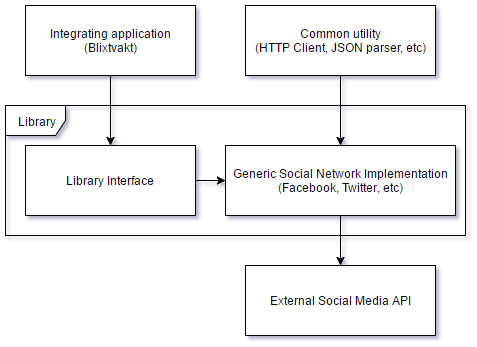
\includegraphics[width=\columnwidth]{LibraryImplementation.png}
	\caption{Architectural overview of library and use case}
	\label{fig:architecturalOverview}
\end{figure}
Our library mainly consist of two parts, see figure~\ref{fig:architecturalOverview}. Where the library interface is what the users are in contact with when interacting with our library. This interface is an abstraction
of a generic social network API. The Generic Social Network Implementation is the actual implementation of each social media platform and acts as the middleware between the interface and the 
external social media platforms.
The internals of each implementation might differ greatly. To as great a degree as possible, we will use existing libraries which are either official or come officially recommended by the API vendor, in order to save time
and avoid reimplementing functionality which is already available and suites our purpose.

The already existing libraries we used are:
\begin{itemize}
	\item twitter4j (http://twitter4j.org/)
	\item facebook4j (https://facebook4j.github.io/)
	\item jumblr (https://github.com/tumblr/jumblr)
\end{itemize}
\subsection{Evaluation}
The evaluation of our library consists of three parts. Throughout the project we have used SonarQube to analyze the quality and maintainability of our code, which is the first part. As for the second, once we have finished
implementing two APIs, we attempted to implement a third, to test the flexibility of the library interface. The third part involves creating a small application which utilizes the library. When selecting the functionality 
of the application we looked at what common denominators was shared between the different plaforms, that might be suitable. This will gave us a hands-on experience on how easy our library is to use in practice and the more 
analytical aspect gained from the SonarQube analysis.

When integrating our library into our test application, we mainly focused on if we felt that there was anything lacking, or if something was not working as intended. If we felt the need to go back and
change the source code of the library, or its interfaces, the result is deemed unsatisfactory. 

\section{Results}
\subsection{Social Networks Selection}
When looking at social media APIs we found that out of the 22 networks from our list\autocite{STATISTA_LEADING_SOCIAL_NETWORKS}, 10 were geographically irrelevant for our study as many of these were
niched at the Asian market, primarily the Chinese one. We then narrowed it down further to networks with APIs which shared a lot of common functionality, see Appendix A, making them more appropriate for the core idea
of our study. Given that the time of the project is finite we chose to look at the top four platforms with good functionality, where Facebook and Messenger was regarded as a single platform.
\begin{itemize}
	\item Facebook
	\item Instagram
	\item Tumblr
	\item Twitter
\end{itemize}

\subsubsection{Comparison}
While comparing APIs functionality we found out that these differ both in how well developed they are as well as how much functionality they offer. Out of the top four platforms facebook and twitter
had the most well developed APIs, as well as libraries developed by the same developer. Making these our top priority. For the last two platforms we chose to prioritize Tumblr over Instagram considering
it had an official library written in java, which would make it faster for us to implement into our own library. As such, our final prioritization was as follows:
\begin{enumerate}
	\item Facebook
	\item Twitter
	\item Tumblr
	\item Instagram
\end{enumerate}

\subsection{Implementation}
In terms of tools used, no implementation compromises had to be made to suite our configuration. Although the library has few dependencies, using Maven made the project significantly more portable, and outside of the
initial startup and configuration, handling dependencies proved to be no issue, even when switching between workstations.

For SonarQube, our original intention was to use it for evaluation of the end result, but it proved more useful during the implementation as well. When committing the code to our git repository, SonarQube would automatically
pull the code and analyze it. As such, we always had a current idea of the state of the quality of the implementation, and we occasionally took the time to correct issues SonarQube reported. A plugin called SonarLint\footnote{http://www.sonarlint.org/},
developed by SonarQube, was also available for IntelliJ IDEA, which uses a more basic rule set than the SonarQube service, but allowed us to avoid many of the most common mistakes, such as unnecessary package imports,
which may not directly impact the usefulness of the library, but results in cleaner, and more easily worked with, code.

\subsection{Work Method}
Using Test Driven Development helped in many cases to give a better understanding at the problem each function is meant to solve. This was the most useful when writing functions which have no side effects, as it allows
for clearer sets of inputs and outputs to and from the function. In essence, writing the tests firsts forced us to write the functions in a way that made them easier to test, and functions which were easy to test also
turned out to be easier to understand.

At the start of the project we set out to document first as to make the documentation reach a higher quality. As our library mainly consists of already documented functionality in most cases this were merely duplicate
information and did not impact our own documentation in any meaningful way.

\subsection{Design}
For two of our chosen platforms, Facebook and Twitter, third-party library implementations of the respective APIs were available. While using these libraries significantly reduced the workload, some compromises had to
be made. One of the two, facebook4j, is completely synchronous, which meant the other implementations had to be synchronous as well in order to be generalized properly.

As the goal was to generalize the social network APIs, we had to look for the lowest common denominator. This meant that the classes for users and posts only supported the very most basic functionality, such as getting
their id, name and biography. Other functionality, such as getting the friends of a user, had to be relegated to API-specific classes, due to the way friendships work on different networks. An example would be Facebook,
where friendship is mutual, while the closest equivalent on Twitter is follow, which can be one-sided. On the other hand, Facebook also has a concept of follow, which is not accessible through the API, and thus Facebook
friends can not be generalized together with the Twitter follow concept.

In some cases, in particular for Facebook, functionality which is available on the site and library users would expect to be present in the library, is not available in the APIs. This is largely in regards to functionality
which could potentially be used to spam or otherwise inconvenience regular users, such as sending friend requests. Some functionality is available, but has additional rules for usage, such as direct messaging. In this case,
users are required to start the conversation, to avoid the chat being used as a system for notifications or ads. This does also mean that the usefulness of chat functionality is significantly reduced in the simple REST API
we intended the library to be, and we decided to leave it out of the library, as it would be more suitable for libraries with this specific purpose.

\subsection{Evaluation}
\subsubsection{SonarQube}
SonarQube proved to be more useful during the implementation process than as an evaluation tool after the implementation was complete. The most useful feature for us was that of code coverage. Code coverage is a somewhat controversial
metric, as it only ensures that the code has been run, but does prevent tests from always using happy paths. Nonetheless, it helped visualize which parts of the code had gone untested, mostly due to human error. It also helped avoiding
bugs, such as using the == operator instead of equals for string comparison, which is usually gives an undesirable result in Java. However, as for evaluation of the end result of the implementation, SonarQube did not prove all that useful,
as the project was simply not large enough in scope to produce a large number of unfixable issues. SonarQube attempt to quantify the complexity of the code, but as the majority of the code written by us simply wraps the libraries we used,
most of the code is of very low complexity. There were also cases where SonarQube considered the complexity to be very high, such as when using Switches with many cases, even though the cases were in actuality very simple and easy to reason about.

\subsubsection{Third API implementation}
As for the second part of our evaluation, once the implementation of Twitter and Facebook was done, we attempted to add Tumblr to our library. This forced some changes to the library interface. One example is where the follower count of users.
For Twitter, this was always accessible, and would always return an integer. In the Facebook API, this is not available at all, and thus always throws an exception. As such, the non-nullable type \textit{int} was chosen as the return type of
the getFollowersCount function in the interface. However, for Tumblr, this functionality \textit{may} be available, depending on the user's settings. If the user has chosen to not make this number available, the API will instead return null, making in
incompatible. Because of this, we had to change the return type to \textit{Integer}. While this may seem like a minor change, it is in fact a breaking change, and would have forced any existing users of the library to make changers in the own code; in
particular, change the types of the variables handling the returned data, and make null checks.

\subsubsection{Test Application}
For the last part of our evaluation, we built a small application to test actually using the library. During the implementation of our test program we found that a lot of the shared functionality was not suitable for generalization. The 
application ended up being a smaller post publisher\footnote{https://github.com/Astol/smlevaluation} that fetched data from reddit\footnote{https://www.reddit.com/dev/api/}, and then republished it on our different platforms. When developing
the application we did not feel like there was anything we had to go back and change in our library for it to work. The development was very straightforward and our library was easy to use.

\section{Discussion}
In this part we will first discuss our findings mentioned in the result chapter and follow up with talking about our chosen method of approach.

\subsection{Method}
\subsubsection{Social media selection}
During this study we have worked against social media networks that have been deemed geographically relevant for the European market. When looking at the top platforms in social media today\autocite{STATISTA_LEADING_SOCIAL_NETWORKS}, many were discarded
because of this. There are several widely used platforms that fall under the Asian market that did not get any attention in this paper. This might affect the general outcome as these might have APIs more suitable for a generic social media library
than the ones used in this study. Although the ones we used represent some of the more popular platforms it might not necessarily mean that it is true for every platform.

\subsubsection{Existing libraries}
In this study we have chosen to use already existing libraries for different social media APIs, when including them into our own library. We did this as a timesaver as to be able to include more platforms in our study, but this also adds another layer of
abstraction to our library. Not only are we dependant on updates from the APIs themselves, but also on the libraries. Worst case scenario is one of these libraries stops being maintained and means that everything needs to be reimplemented for that social
media. For this reason, rather than directly reusing library classes such as User or Post, we wrote our own wrapper classes, in order to decouple the libraries from the integrating application, and as such make a potential transition from one library to
another easier.

\subsubsection{Document first}
In our work process we set out to document first, as one of the recommendations for achieving a higher quality on the end product described by Henning\autocite{Henning:2007:ADM:1255421.1255422}. This was mostly for this project not very relevant. As we implemented functionality already written, both in the APIs and in the used libraries, we did not design much functionality ourselves. This meant a lot of rewriting documentation from the APIs and libraries we ourselves used. There were instances when it served it’s purpose, but
for the overall project it did not affect our result in any significant way.

\subsubsection{Test Driven Development}
Due to poor documentation, both in regards to the APIs as well as the libraries, it was often difficult to write tests first. On many occasions, there were no examples of how the returned data was formatted, or what would happen if e.g. there was an attempt to fetch
a post with a specified ID, but no such post was found. For two libraries, this simply returned null. For the third library, an exception was instead thrown. Neither of these two behaviors were documented, but we instead had to choose between directly reading the
source code, which turned out to be a very time consuming task, or simply write the prototype of the function, use the debug tools to check exactly what was returned, and then modify the function to accommodate it. As such, we were often unable to write tests first,
as we had no idea how to format our tests before the function was already written.

\subsection{Result}
\subsubsection{Implementation and work method}
In regards to the actual implementation work of the library, very few issues came up. As we relied heavily on third party libraries for the API implementations, Maven proved very useful for dependency handling. Using a full-featured IDE such as IntelliJ IDEA also
helped with debugging, which was particularly useful as some functionality in the library was often poorly documented and had few to no examples of the formatting of the data returned.

\subsubsection{Design}
The result proved to be more negative than our initial expectations. Although it may seem at a glance that a lot of functionality was present in several APIs, as can be seen in Appendix A, their actual implementation often made them
unsuitable for generalization. Examples of this includes check-ins for posts, where some APIs only allows a general area, like a city, where others use more specific locations, such as a movie theatre, identified by a specific Place ID. In general,
it appears the APIs are built much more with the intention of fetching information rather than creating or modifying. In many cases, functionality has previously been available in the APIs, but have later been removed in order to combat spam and other
abuse. This is noticeable in particular for Facebook, where much of the functionality is still present in the documentation, but tagged as either deprecated or already removed, despite the functionality still being available on the actual Facebook
site and mobile applications.

\subsubsection{Evaluation bias}
In our third evaluation we developed an application, using our library. Due to the fact that we wrote the application ourselves, and interpreted the result, this might lead to a degree of bias. As we as developers of the library we might
have felt functionality was obvious and easily understood, where a test including third party participants might have proven otherwise.

\section{Future work}
As this paper was limited in time there are some aspects that could be further researched to give a broader view on the practicality of a generic social media library. The main focus of these being on to including more social media platforms
and analyze a broader spectrum of platforms. This would give a more accurate view on the practicality in question. 

\section{Conclusion}
As for the general conclusion of this study we have deemed the end result to be unsatisfactory due to the current state of APIs. Where the APIs share functionality this seems to be mostly coincidental rather than deliberate. The different
platforms vary greatly, both in how they logically are built and on what functionality they choose to offer in their APIs. In some cases functionality that once was available has been removed. This discontinuation of functionality also
raises further worries for the future, as it could be possible that functionality critical to the integrating application may be removed, with no alternative being added.

As we did not research the whole market of social media we see the need for further study to see if this is true as a whole. But for this study we must conclude that this is regrettably not feasible at the present time. Our recommendation
for anyone wishing to integrate social media into their applications would instead be to research which social networks are the most suitable, and then use the existing individual libraries to integrate the desired functionality.

\printbibliography[notcategory=ignore]
\clearpage
\appendixpage
\section{Appendix A: API Support Tables}
\label{app:apisupport}
\begin{figure}[htb]
	\rotatebox[origin=c]{-90}{
 	\begin{minipage}{7in}
	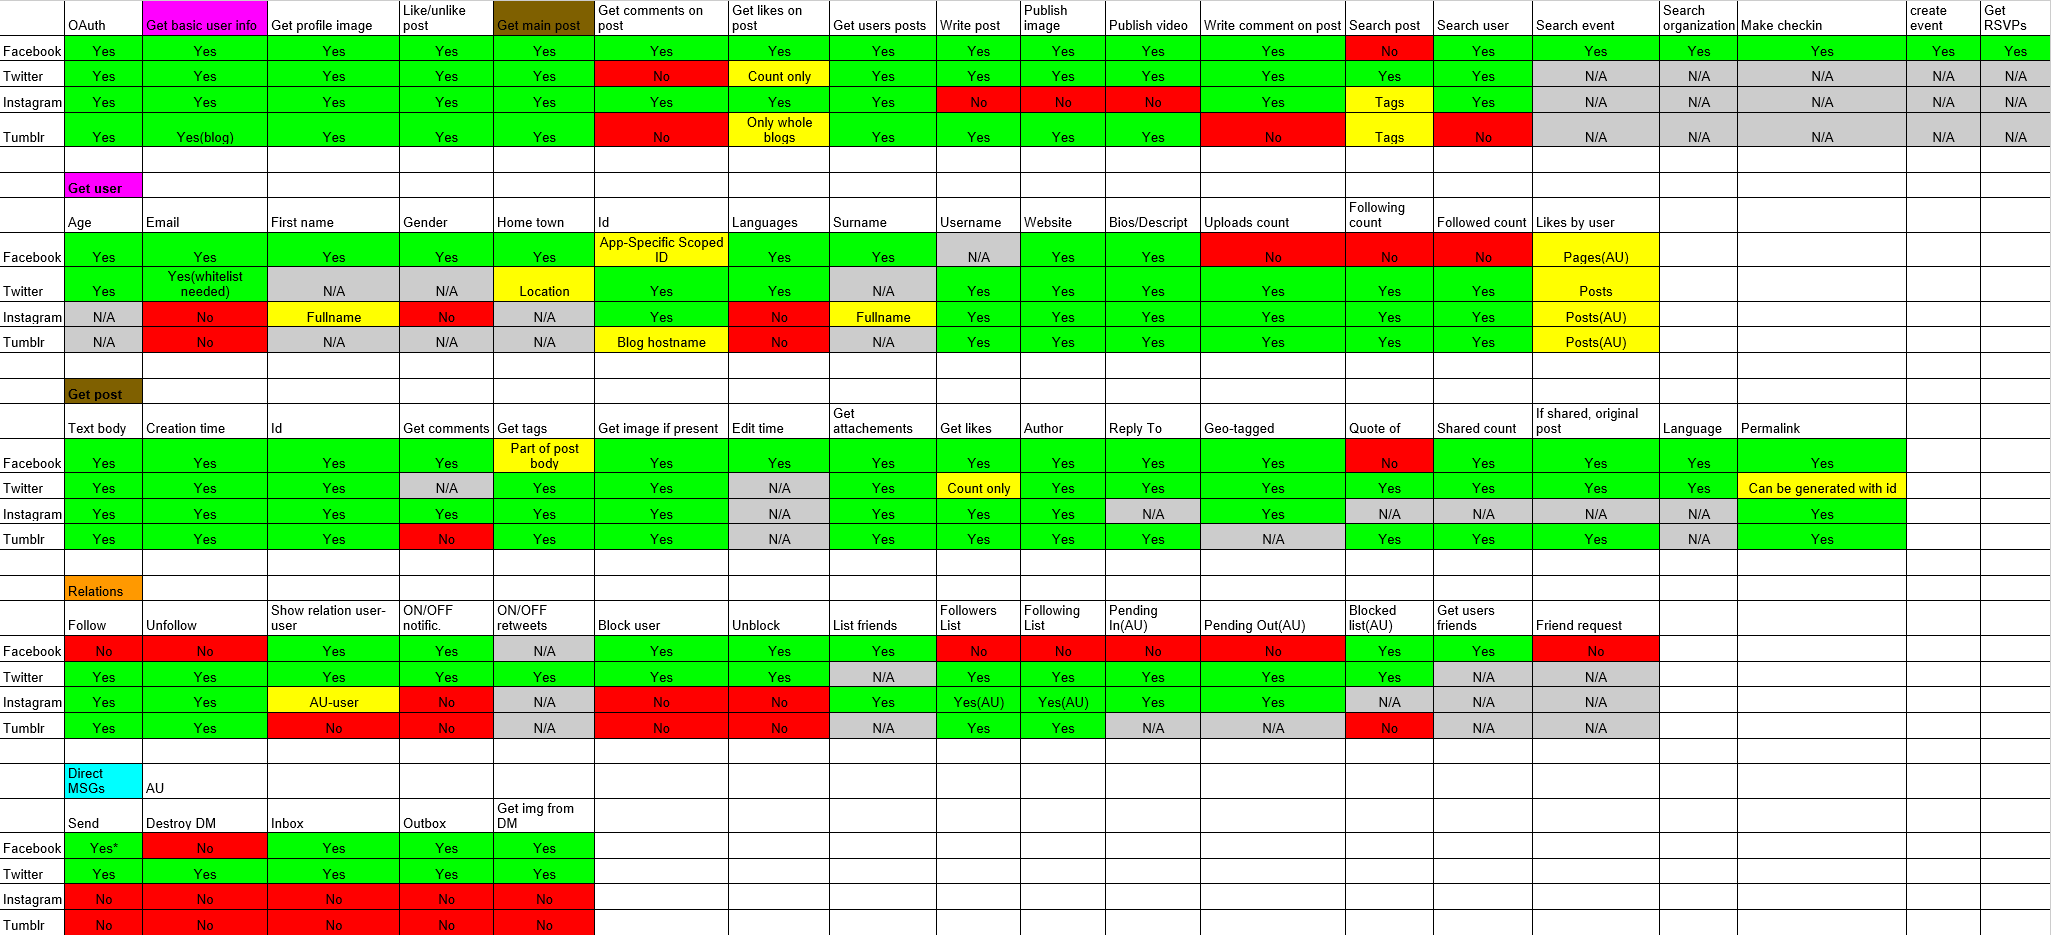
\includegraphics[width=\paperwidth]{tables.png}
	\caption{Overview of functionality supported by different APIs. Green indicates the functionality is fully available through the API. Yellow indicates functionality is partly available. 
		Red indicates functionality is present on the platform, but not available through the API. Gray indicates the functionality is not a part of the platform, and is as such not applicable. \\
		* For Facebook, direct message conversations must be initiated and kept alive by the conversation target in order to be used through the API.
	}
	\label{fig:apisupporttables}
	\end{minipage}
	}
\end{figure}
\end{document}
